\section{Statechart diagrams}
Statechart diagrams are a useful way to get an overview over the lifetime of objects in the problem domain.
This chapter describes contains the state chart diagram of objects whose behaivour is both interesting and unique to the project.
Due to the nature of the application, it being very focused on basic CRUD operations, there is not a lot of interesting activity going on in the way of state.
\subsection{Approval Request}
The approval request is one of the most central concepts in the application.
When someone wants to create a new version of a document, they instantiate an approval request, which has a version object attached.
When the change is approved, it will append the version to the document object.
% kan der ikke også være "denied" iteration ?
% i den sidste state kan den muligvis hedde new version released?

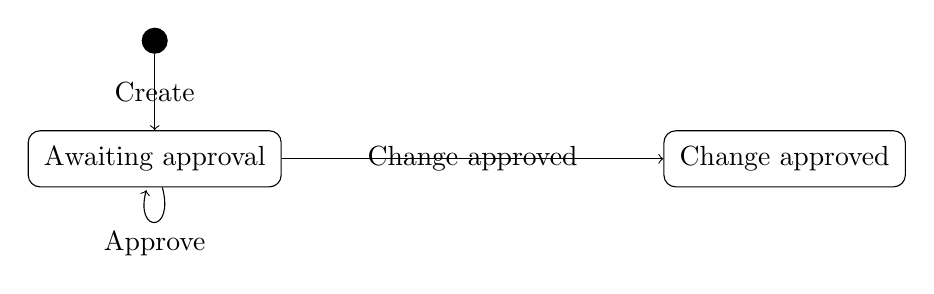
\begin{tikzpicture}[round/.style={rounded corners=1.5mm,minimum width=1cm,inner sep=2mm,above right,draw,align=left}]

	\node[circle, fill=black,minimum size=3pt] (start) {};
	\node[round] (await) [below of=start, node distance=1.5cm] {Awaiting approval};
	\path[->] (start) edge node {Create} (await);
	\path[->] (await) edge [loop below] node {Approve} (await);
	\node[round] (approved) [right of=await, node distance=8cm] {Change approved};
	\path[->] (await) edge node {Change approved} (approved);

	%\draw[fill=white] circle[radius = 7pt, below of=approved, node distance=1cm];
	%\node[circle, fill=black,minimum size=3pt] (end) [below of=approved, node distance=1cm] {};


\end{tikzpicture}

\subsection{Department}
A department is an organisational unit, used to administrate which users are attached to which documents.
As such, you can create a department, add users to it, and add documents to it.
You can also remove both in the same way.
One of the most important functions of the department is the abillity for it to notify all the users which are attached to it of a new version of a document.
% er det ikke mere assign user og assign  document end add user og add document? 
% tænker om unassign muligvis også skal med? 

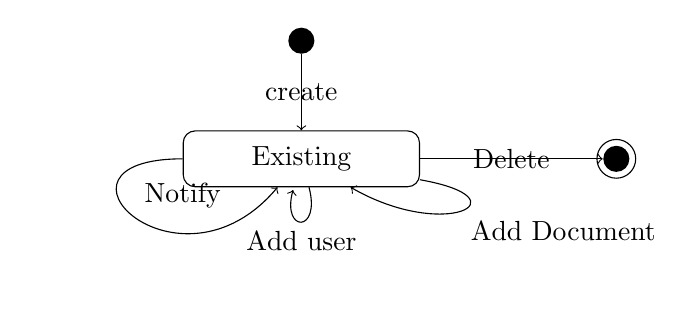
\begin{tikzpicture}[round/.style={rounded corners=1.5mm,minimum width=1cm,inner sep=2mm,above right,draw,align=left}]

	\node[circle, fill=black,minimum size=3pt] (start) {};
	\node[round, minimum width=3cm] (await) [below of=start, node distance=1.5cm] {Existing};
	\path[->] (start) edge node {create} (await);
	\path[->] (await) edge [loop below] node[auto] {Add user} (await);
	\path[->] (await) edge [loop below, out=350, in=330, looseness=4] node[auto] {Add Document} (await);
	\path[->] (await) edge [loop below, out=180, in=230, looseness=4] node[auto] {Notify} (await);

	\draw[fill=white] circle[radius = 7pt, right of=await, node distance=4cm];
	\node[circle, fill=black,minimum size=3pt] (end) [right of=await, node distance=4cm] {};
	\path[->] (await) edge node {Delete} (end);


\end{tikzpicture}

\subsection{Version}
A version is another central concept in the application.
As mentioned before, the handbook consists of documents, and each document can have multiple versions.
And thus, after creation, version objects are supposed to be quite immutable once created, as to preserve the history of individual documents.
% mangler der ikke efter approved state en released version eller noget, så det er tydeligt at reader bruger nu kan se den nye version

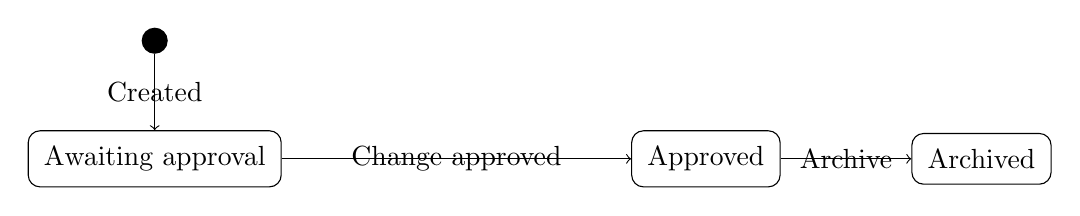
\begin{tikzpicture}[round/.style={rounded corners=1.5mm,minimum width=1cm,inner sep=2mm,above right,draw,align=left}]

	\node[circle, fill=black,minimum size=3pt] (start) {};
	\node[round] (await) [below of=start, node distance=1.5cm] {Awaiting approval};
	\path[->] (start) edge node {Created} (await);
	\node[round] (approved) [right of=await, node distance=7cm] {Approved};
	\path[->] (await) edge node {Change approved} (approved);
	\node[round] (archived) [right of=approved, node distance=3.5cm] {Archived};
	\path[->] (approved) edge node {Archive} (archived);

	%\draw[fill=white] circle[radius = 7pt, below of=approved, node distance=1cm];
	%\node[circle, fill=black,minimum size=3pt] (end) [below of=approved, node distance=1cm] {};


\end{tikzpicture}
